%% This is file `gabaritmem.tex',
%% generated with the docstrip utility.
%%
%% The original source files were:
%%
%% dms.dtx  (with options: `memoire,gabarit')
%% Example TeX file for the documentation
%% of the jurabib package
%% Copyright (C) 1999, 2000, 2001 Jens Berger
%% See dms.ins  for the copyright details.
%%
%%% ====================================================================
%%%  @LaTeX-file{
%%%     filename        = "dms.dtx",
%%%     author    = "Nicolas Beauchemin, Damien Rioux-Lavoie, Victor Fardel, Jonathan Godin",
%%%     copyright = "Copyright (C) 2000 , DMS
%%%                  all rights reserved.  Copying of this file is
%%%                  authorized only if either:
%%%                  (1) you make absolutely no changes to your copy,
%%%                  including name; OR
%%%                  (2) if you do make changes, you first rename it
%%%                  to some other name.",
%%%     address   = "Département de Mathématiques et de Statistique",
%%%     telephone = "514-343-6705",
%%%     FAX       = "514-343-5700",
%%%     email     = "aide@dms.umontreal.ca (Internet)",
%%%     keywords  = "latex, amslatex, ams-latex, theorem",
%%%     abstract  = " Ce fichier est un package conçu pour être
%%%                  utilisé avec la version de LaTeX2e 1995/06/01. Il
%%%                  est prévue pour la classe ``amsbook''. Il en
%%%                  modifie le format des pages, l'entête des
%%%                  sections, etc, afin d'être  conforme au modèle de
%%%                  mémoire de maîtrise de l'Université de
%%%                  Montréal. Finalement ce fichier est grandement
%%%                  inspiré du fichier amsclass.dtx.",
%%%     docstring = "The checksum field contains: CRC-16 checksum,
%%%                  word count, line count, and character count, as
%%%                  produced by Robert Solovay's checksum utility."}
%%%  ====================================================================

%% Pour voir les accents de ce fichier, assurez-vous que votre
%% éditeur de texte lise le fichier en utf-8!

%% La classe <dms> est construite au-dessus de <amsbook>, donc
%% <amsmath>, <amsfonts> et <amsthm> sont automatiquement chargés.
%% Pour un mémoire
\documentclass[12pt,twoside,maitrise]{dms}
%% Pour une thèse
%%\documentclass[12pt,twoside,phd]{dms}

\usepackage[utf8]{inputenc} %Obligatoires
\usepackage[T1]{fontenc}    %
\usepackage{tabularx}


%% <lmodern> incorpore les fontes en T1, pour
%% faciliter le dépôt final. Ceci n'est pas la
%% seule option :
%%  1. Si cm-super est installé, vous pouvez enlever <lmodern>
%%     (à ce moment, la police est un peu plus fidèle
%%      au Computer Modern orginal);
%%  2. Si vous avez une police préférée, par exemple,
%%     <times> ou <euler> ou <mathpazo> (et bien d'autres),
%%     alors vous pouvez remplacer <lmodern> ci-bas.
%% Par contre, si vous faîtes face à un problème d'encapsulation
%% lors dépôt final, il se peut que la solution soit d'utiliser <lmodern>.
%% (Parfois le problème est au niveau de l'installation, donc
%%  essayez de compiler sur un autre ordinateur sur lequel vous êtes
%%  certain·e que l'installation est bonne.)
\usepackage{lmodern}
\DeclareSymbolFont{largesymbols}{OMX}{cmex}{m}{n}

%% Il n'est pas nécessaire d'utiliser <babel>, car
%% les commandes intégrées par la classe <dms>
%% \francais et \anglais font le travail. Néanmoins,
%% certains autres packages nécessitent <babel> (comme
%% <natbib>), donc simplement enlever les % devant <babel>
%% dans ce cas. Attention! Certains packages sont sensibles
%% à l'ordre dans lequel ils sont chargés.
\francais % or
%%\anglais
%%
%%\usepackage[english,frenchb]{babel}

 % ENGLISH OPTION
 % If you call \anglais here before the \begin{document},
 % all the chater's header will be in english, even if you
 % call \francais. To change this, use
 % \entetedynamique

%% La commande \sloppy peut avoir des effets étranges sur les
%% lignes de certains paragraphes.  Dans ce cas, essayez \fussy
%% qui suppresse les effets de \sloppy.
%% (\fussy est normalement le comportement par défaut.)
%% On redéfinit \sloppy, pour tenter de réduire les comportements
%% étranges. Le seul changement apporté à la version originale
%% est la valeur de \tolerance.
\def\sloppy{%
  \tolerance 500%  %9999 dans LaTeX ordinaire, mauvaise idée.
  \emergencystretch 3em%
  \hfuzz .5pt
  \vfuzz\hfuzz}
\sloppy   %appel de \sloppy pour le document
%%\fussy  %ou \fussy

%% Packages utiles.
\usepackage{graphicx,amssymb,subfigure,icomma}
%% icomma       permet d'écrire les nombres décimaux en
%%                  français (p.ex. 1,23 plutôt que 1.23)
%% subfigure    simplifie l'inclusion de figures côtes-à-côtes

%% Packages parfois utiles.
\usepackage{dsfont,mathrsfs,color,url,verbatim,booktabs}
%% dsfont       symboles mathématiques \mathds
%% mathrsfs     plus de symboles mathématiques \mathscr
%% color        pour utiliser des couleurs (comparer avec <xcolor>)
%% url          permet l'écriture d'url
%% verbatim     pour écrire du code ou du texte tel quel
%% booktabs     plus de macros pour faire les tableaux
%%                  (voir documentation du package)

%% pour que la largeur de la légende des figures soit = \textwidth
\usepackage[labelfont=bf, width=\linewidth]{caption}

%% les 3 lignes suivante servent à l'affichage de l'index
%% dans le visionneur de pdf. <hyperref> et <bookmark>
%% devraient être les dernier package a être chargé,
%% donc chargez vos packages avant.
\usepackage{hyperref}  % Ajoute les hyperlien
\hypersetup{colorlinks=true,allcolors=black}
\usepackage{hypcap}   % Corrige la position du lien pour les images
\usepackage{bookmark} % Remédie à des petits problème
                      % de <hyperref> (important qu'il
                      % apparaisse APRÈS <hyperref>)

  % Enlever les commentaires du prochaine \hypersetup et
  % le remplir avec l'information pertinente.
  % Ceci ajoute des « méta-données » au pdf.  C'est optionnel,
  % mais recommandé. Vous pouvez voir ces méta-données en
  % ouvrant un visionneur de pdf et en cherchant les propriétés
  % du pdf. (Vous pouvez aussi tapez ' pdfinfo <nom-du-pdf> '
  % dans un terminal.) Ces données sont utiles, par exemple,
  % pour augmenter les chances qu'un algorithme de recherche
  % trouve votre document sur Internet, une fois diffusé.
%%\hypersetup{
%%  pdftitle = {Titre de la thèse / du mémoire},
%%  pdfauthor = {auteur·e},
%%  pdfsubject = {Ex: Transformation de Fourier ; régressions linéaires ; ... },
%%  pdfkeywords = {Ex: mathématiques, statistiques, groupes, variables aléatoires,...}
%%}

%% Définition des environnements utiles pour un mémoire scientifique.
%% La numérotation est laissée à la discrétion de l'auteur·e. L'exemple
%% illustré ici produit « Définition x.y.z »
%%   x = no. chapitre
%%   y = no. section
%%   z = no. définition
%% et la numérotation des corollaires, définitions, etc. se fait
%% successivement.
%%
%% Les macros \<type>name sont telles qu'ils suivent
%% la langue actuelle. (P.ex. si \francais est utilisé,
%% alors \begin{theo} va faire un Théorème et si \anglais
%% est utilisé, \begin{theo} fera un Theorem.)
%%
\newtheorem{cor}{\corollaryname}[section]
\newtheorem{theo}[cor]{\theoremname}
\newtheorem{prop}[cor]{Proposition}
\newtheorem{lem}[cor]{\lemmaname}
\theoremstyle{definition}
\newtheorem{deff}[cor]{\definitionname}
\newtheorem{ex}[cor]{\examplename}
\newtheorem{rem}[cor]{\remarkname}
\newtheorem{algo}[cor]{\algoname}
%% NOTE : Il peut être commode de redéfinir \the<type> pour
%% obtenir la numérotation désirée. Par exemple, pour
%% que les corollaires soit numérotés #section.#sous-section.#sous-sous-section.#paragraphe.#corollaire,
%% on fait
%% \renewcommand\thecor{\theparagraph.\arabic{cor}}

%%%
%%% Si vous préférez que les corollaires, définitions, théorèmes,
%%% etc. soient numérotés séparément, utilisez plutôt un bloc de
%%% commandes de la forme :
%%%



%%\newtheorem{cor}{\corollaryname}[section]
%%\newtheorem{deff}{\definitionname}[section]
%%\newtheorem{ex}{\examplename}[section]
%%\newtheorem{lem}{\lemmaname}[section]
%%\newtheorem{prop}{Proposition}[section]
%%\newtheorem{rem}{\remarkname}[section]
%%\newtheorem{theo}{\theoremname}[section]

%%
%% Numérotation des équations par section
%% et des  tableaux et figures par chapitre.
%% Ceci peut être modifié selon les préférences de l'utilisateur.
\numberwithin{equation}{section}
\numberwithin{table}{chapter}
\numberwithin{figure}{chapter}

%%
%% Si on veut faire un index, il faut décommenter la ligne
%% suivante. Ajouter des mots à l'index avec la commande \index{mot cle} au
%% fur et à mesure dans le texte.  Compiler, puis taper la commande
%% makeindex pour creer les indexs.  Après une nouvelle compilation,
%% vous aurez votre index.
%%

%%\makeindex

%% Il est obligatoire d'écrire à double interligne
%% ou à interligne et demi. On peut soit utiliser
%% le package <setspace> ou \baselinestretch.
%% Le package a tendance a créé des grands blancs,
%% le gabarit décourage son utilisation, mais il en
%% reste à la discrétion de l'utilisateur·e.
%% \usepackage[onehalfspacing]{setspace}
 % ou
\renewcommand{\baselinestretch}{1.286} %Interligne et demi (environ 18pt (12pt+6pt) entre les lignes)
%%%%%%%%%%%%%%%%%%%%%%%%%%%%%%%%%%%%%%%%%%%%%%%%%%%%%%%%%%%%
%%%%%%%%%%%%%%%%%%%%%%%%%%%%%%%%%%%%%%%%%%%%%%%%%%%%%%%%%%%%
%%%%%%%%%%                                     %%%%%%%%%%%%%
%%%%%%%%%% D é b u t    d u    d o c u m e n t %%%%%%%%%%%%%
%%%%%%%%%%                                     %%%%%%%%%%%%%
%%%%%%%%%%%%%%%%%%%%%%%%%%%%%%%%%%%%%%%%%%%%%%%%%%%%%%%%%%%%
%%%%%%%%%%%%%%%%%%%%%%%%%%%%%%%%%%%%%%%%%%%%%%%%%%%%%%%%%%%%
\begin{document}

%%
%% Voici des options pour annoter les différentes versions de votre
%% mémoire. La commande \brouillon imprime, au bas de chacune des pages, la
%% date ainsi que l'heure de la dernière compilation de votre fichier.
%%
%%\brouillon
%%
%%
%% \version est la version de votre manuscrit
%%
\version{1}

%%------------------------------------------------- %
%%              pages i et ii                       %
%%------------------------------------------------- %

%%%
%%% Voici les variables à définir pour les deux premières pages de votre
%%% mémoire.
%%%

\title{Préentraînement d'un modèle ELECTRA}

\author{Simon Théorêt}

\copyrightyear{2025}

\department{Département d'informatique et de recherche opérationnelle}

\date{7 février 2025} %Date du DÉPÔT INITIAL (ou du 2e dépôt s'il y a corrections majeures)

\sujet{informatique, \orientation{apprentissage automatique}}
%%\orientation{orientation}%Ce champ est optionnel
%%
%% Voici les disciplines possibles (voir avec votre directeur):
%% \sujet{statistique},
%% \sujet{mathématiques}, \orientation{mathématiques appliquées},
%% \orientation{mathématiques fondamentales}
%% \orientation{mathématiques de l'ingénieur} et
%% \orientation{mathématiques appliquées}

\president{Nom du président du jury}

\directeur{Nom du directeur de recherche}

%%\codirecteur{Nom du 1er codirecteur}         % s'il y a lieu
%%\codirecteurs{Nom du 2e codirecteur}         % s'il y a lieu

\membrejury{Nom du membre de jury}

%%\examinateur{Nom de l'examinateur externe}   %obligatoire pour la these

%% \membresjury{Deuxième membre du jury}  % s'il y a lieu

%%  \plusmembresjury{Troisième membre du jury}    % s'il y a lieu

% Cette option existe encore, mais elle n'a plus sa place
% dans la page titre. L'utiliser seulement si le directeur
% insiste...
%%\repdoyen{Nom du représentant du doyen} %(thèse seulement)

%%
%% Fin des variables à définir. La commande \maketitle créera votre
%% page titre.

%% Pour mettre bouton qui mène à la page titre
%% dans le visionneur de pdf. Peut être enlever.
\pdfbookmark[chapter]{Couverture}{PageUn}

\maketitle

% Pour générer la deuxième page titre, il faut appeler à nouveau \maketitle
% Cette page est obligatoire.
\maketitle

%%------------------------------------------------- %
%%              pages iii                           %
%%------------------------------------------------- %

\francais

\chapter*{Résumé}
Le logiciel Antidote permet de corriger des textes en français et en anglais.
Il détecte plusieurs milliers de types d’erreurs orthographiques et
grammaticales. Le logiciel dispose d'un modèle ELECTRA capable de détecter
efficacement les erreurs en français. L'équipe de TAL de Druide désire mettre
en place un système similaire pour la langue française . Dans le cadre de ce
stage, le but est de créer un modèle ELECTRA capable de détecter les erreurs
grammaticales en français. Pour ce faire, plusieurs approches ont été testées
et les résultats des derniers modèles sont prometteurs. On remarque entre autre
une hausse importante des performances en introduisant une tâche intermédiaire
et en faisant une recherche d'hyperparamètres.\\

\textit{Mots clés: Apprentissage automatique, Apprentissage profond,
	Apprentissage machine, Traitement de texte, Détection de mot manquants,
	Encodeur, Transformers, BERT, Electra, Réseaux de neurones, Intelligence
	artificielle.}

%%------------------------------------------------- %
%%              pages iv                            %
%%------------------------------------------------- %

%%------------------------------------------------- %
%%        page v --- Table de matieres              %
%%------------------------------------------------- %

% Pour un mémoire en anglais, changer pour
% \anglais. Noter qu'il faut une permission
% pour écrire son mémoire en anglais.
%%\anglais
\francais
% \cleardoublepage termine la page actuel et force TeX
% a poussé les éléments flottant (fig., tables, etc.) sur
% la page (normalement TeX les garde en suspend jusqu'à ce
% qu'il trouve un endroit approprié). Avec l'option <twoside>,
% la commande s'assure que la prochaine page de texte est sur
% le recto, pour l'impression. On l'utilise ici
% pour que TeX sache que la table des matières etc. soit
% sur la page qui suit.
%% TABLE DES MATIÈRES
\cleardoublepage
\pdfbookmark[chapter]{\contentsname}{toc}  % Crée un bouton sur
% la bar de navigation
\tableofcontents
% LISTE DES TABLES
\cleardoublepage
\phantomsection  % Crée une section invisible (utile pour les hyperliens)
\listoftables
% LISTE DES FIGURES
\cleardoublepage
\phantomsection
\listoffigures

%%%%%%%%%%%%%%%%%%%%%%%%%%%%%%%%%%%%%
%% LISTE DES SIGLES ET ABRÉVIATION %
%%%%%%%%%%%%%%%%%%%%%%%%%%%%%%%%%%%%%
%% Il est obligatoire, selon les directives de la FESP,
%% pour une thèse ou un mémoire d'avoir une liste des sigles et
%% des abréviations.  Si vous considérez que de telles listes ne seraient pas
%% pertinentes (si, par exemple, vous n'utilisez aucun sigle ou abré.), son
%% inclusion ou omission est laissé à votre discrétion.  En cas de doute,
%% parlez-en à votre directeur de recherche, le coadministrateur ou au/à la
%% bibliothécaire.
%%
%% Le gabarit inclut un exemple d'une liste « fait à la main ».  Il existe des outils
%% plus sophistiqués si vous devez inclure une multitude de sigles et abréviations.
%% Par exemple, le package <glossaries> peut faire des index élaborés.  Comme
%% son utilisation est technique, il n'y a pas d'exemple directement dans ce gabarit.
%% On invite les gens qui aurait à l'utiliser à lire la documentation officielle,
%% soit en allant sur https://www.ctan.org/, soit en tapant dans un terminal :
%%
%% texdoc glossaries
%%

\chapter*{Liste des sigles et des abréviations}
\begin{twocolumnlist}{.2\textwidth}{.7\textwidth}
	MLM & Modélisation de langage avec masque, de l'anglais
	\textit{Masked Language Modeling}\\
	TAL & Traitement automatique du langage\\
	NER & Reconnaissance d'entitées, de l'anglais
	\textit{Named-Entity Recognition}\\
	DDP & Parallélisme distribué des données, de l'anglais
	\textit{Distributed Data Parallel}\\
	MOE & Mélange d'expertes, de l'anglais
	\textit{Mixture of experts}\\
	TPE & Estimateur de Parzen à base d'arbres, de l'anglais
	\textit{Tree-Structured Parzen Estimator}\\
\end{twocolumnlist}
% Option de colonnes: definir \colun ou \coldeux
%%% Exemple
%%% \def\colun{\bf} % Première colonne en gras
%%% Pour numéroté les entrées, on peut faire
%%% \newcount\abbrlist
%%% \abbrlist=0
%%% \def\plusun{\global\advance\abbrlist by 1\relax}
%%% \def\colun{\plusun\the\abbrlist. }
%%\def\coldeux{\relax}
%% L'environnement <threecolumnlist> existe aussi pour trois colonnes.

%%------------------------------------------------- %
%%              pages vi                            %
%%------------------------------------------------- %

\chapter*{Remerciements}

Je tiens remercier Joss, pour sa précieuse aide tout au long de mon stage. Je
n'aurais pas pu demander un meilleur superviseur. \\
Je remercie aussi Momo pour son support moral constant.

%
% Fin des pages liminaires.  À partir d'ici, les
% premières pages des chapitres ne doivent pas
% être numérotées
%

\NoChapterPageNumber
\cleardoublepage
\pagenumbering{arabic}

%%%%%%%%%%%%%%%%%%%%%%%%%%%%%%%%%%%%%%%%%%%%%%%%%%%%%
%%                                                  %
%%   TEXTE DU MÉMOIRE :  introduction page 1,...    %
%%                                                  %
%%%%%%%%%%%%%%%%%%%%%%%%%%%%%%%%%%%%%%%%%%%%%%%%%%%%%

\setcounter{page}{17} % Resets the page counter to start from 1
\chapter*{Introduction}
Le domaine du traitement automatique des langues connaît une explosion
fulgurante de techniques, de jeux de données et de modèles permettant de
résoudre de nouveaux problèmes. Néanmoins, bon nombre de ces applications
restent hors de portée des organisations désirant mettre en application des
outils d'apprentissages automatique. En effet, la plupart des modèles de
langues récents sont préentraînés sur des corpus majoritairement anglophones,
avec des jetoniseurs spécialisés pour traiter le contenu anglophone. Ces deux
facteurs limitent les modèles préentraînés disponibles ainsi que leur
performance sur des tâches avec un corpus non anglophone.\\

Druide Inc. est une compagnie basée à Montréal dont le principal produit est
Antidote, un logiciel de correction orthographique et grammaticale. Leur
logiciel phare fait déjà usage de l'apprentissage profond pour leur moteur de
correction en anglais, en plus d'utiliser un correcteur symbolique pour
certains types d'erreurs. Le modèle utilisé en production pour la correction en
anglais fait près de 2 corrections sur 3 et représente une part importante du
moteur de correction. L'équipe de Druide désire mettre en place un modèle de
correction similaire, mais adapté à la langue française. En particulier, ils
désirent préentraîner un modèle ELECTRA avec un corpus et un jetoniseur
francophones pour que le modèle puisse détecter les erreurs grammaticales
présentes dans les textes des utilisateurs d'Antidote.\\

Pour la réalisation du projet, nous disposons d'un jeu de données d'environ 40
GB de données non structuré. De plus, l'entraînement du modèle se fait
localement sur une machine ayant accès à 3 NVIDIA RTX A4000, disposant chacune
de 16 GB de mémoire VRAM.


%%------------------------------------------------- %
%%                pages 1                           %
%%------------------------------------------------- %

\chapter{Druide et ELECTRA}
L'équipe de Druide dispose de deux modèles déjà en place pour la correction des
erreurs. Néanmoins, leur modèle en anglais corrige une plus grande gamme
d'erreurs. Druide désire améliorer leur moteur de correction en français à
l'aide de l'apprentissage profond.
% NOTE: Nécessaire?

\section{Contraintes}
Le modèle doit être intégré dans le logiciel principal de Druide, Antidote. Or,
le logiciel Antidote est déployé sur les ordinateurs personnels des usagers.
Cela implique d'importantes contraintes quant aux ressources disponibles pour
l'exécution du modèle, notamment en ce qui à trait à la consommation de
mémoire. De plus, le logiciel Antidote se doit d'être rapide, puisque attendre
plusieurs minutes pour la correction d'un texte volumineux dégrade la qualité
de l'expérience des utilisateurs. En d'autres mots, le modèle doit être rapide
durant l'inférence. Finalement, le logiciel antidote cible deux système
d'exploitation: Windows et MacOS.\@ Le déploiement du modèle sur les machines
des usagers se fait à l'aide des librairies ONNX\cite{onnxruntime} et CoreML.\@
Il est donc nécessaire que le modèle soit supporté par les deux librairies.
En résumé, nous avons des limites quant aux ressources disponibles durant
l'inférence ainsi que des contraintes quant aux couches et modèles utilisables.\\

Ces contraintes ont poussé l'équipe du TAL de Druide à sélectionner
des petits modèles Transformers\cite{vaswani2023attentionneed} avec
encodeur. Ces derniers contiennent environ 14 millions de paramètres.

\section{Méthode de préentraînement ELECTRA}

La méthode ELECTRA\cite{clark2020electrapretrainingtextencoders} est une
méthode inspirée de la modélisation de langage avec masque (Masked Language
Modeling; MLM), mais qui se veut plus efficace et rapide que le MLM. La méthode
ELECTRA consiste à entraîner deux modèles: un petit modèle, appelé le
générateur, et le modèle final, appelé le discriminant. Le générateur reçoit
des jetons masqués et doit prédire quel était le jeton original situé à la
position du masque. Les prédictions du modèle sont échantillonnés, de façon à
obtenir une nouvelle séquence, potentiellement différente de la séquence
originale. Le discriminant reçoit la nouvelle séquence et à pour tâche de
prédire quels jetons sont corrompus et lesquels n'ont pas été modifiés par le
générateur. Seul le discriminant est réutilisé pour l'affinage. La méthode est
visualisée dans la figure \ref{fig:electra}.

\begin{figure}
	\begin{center}
		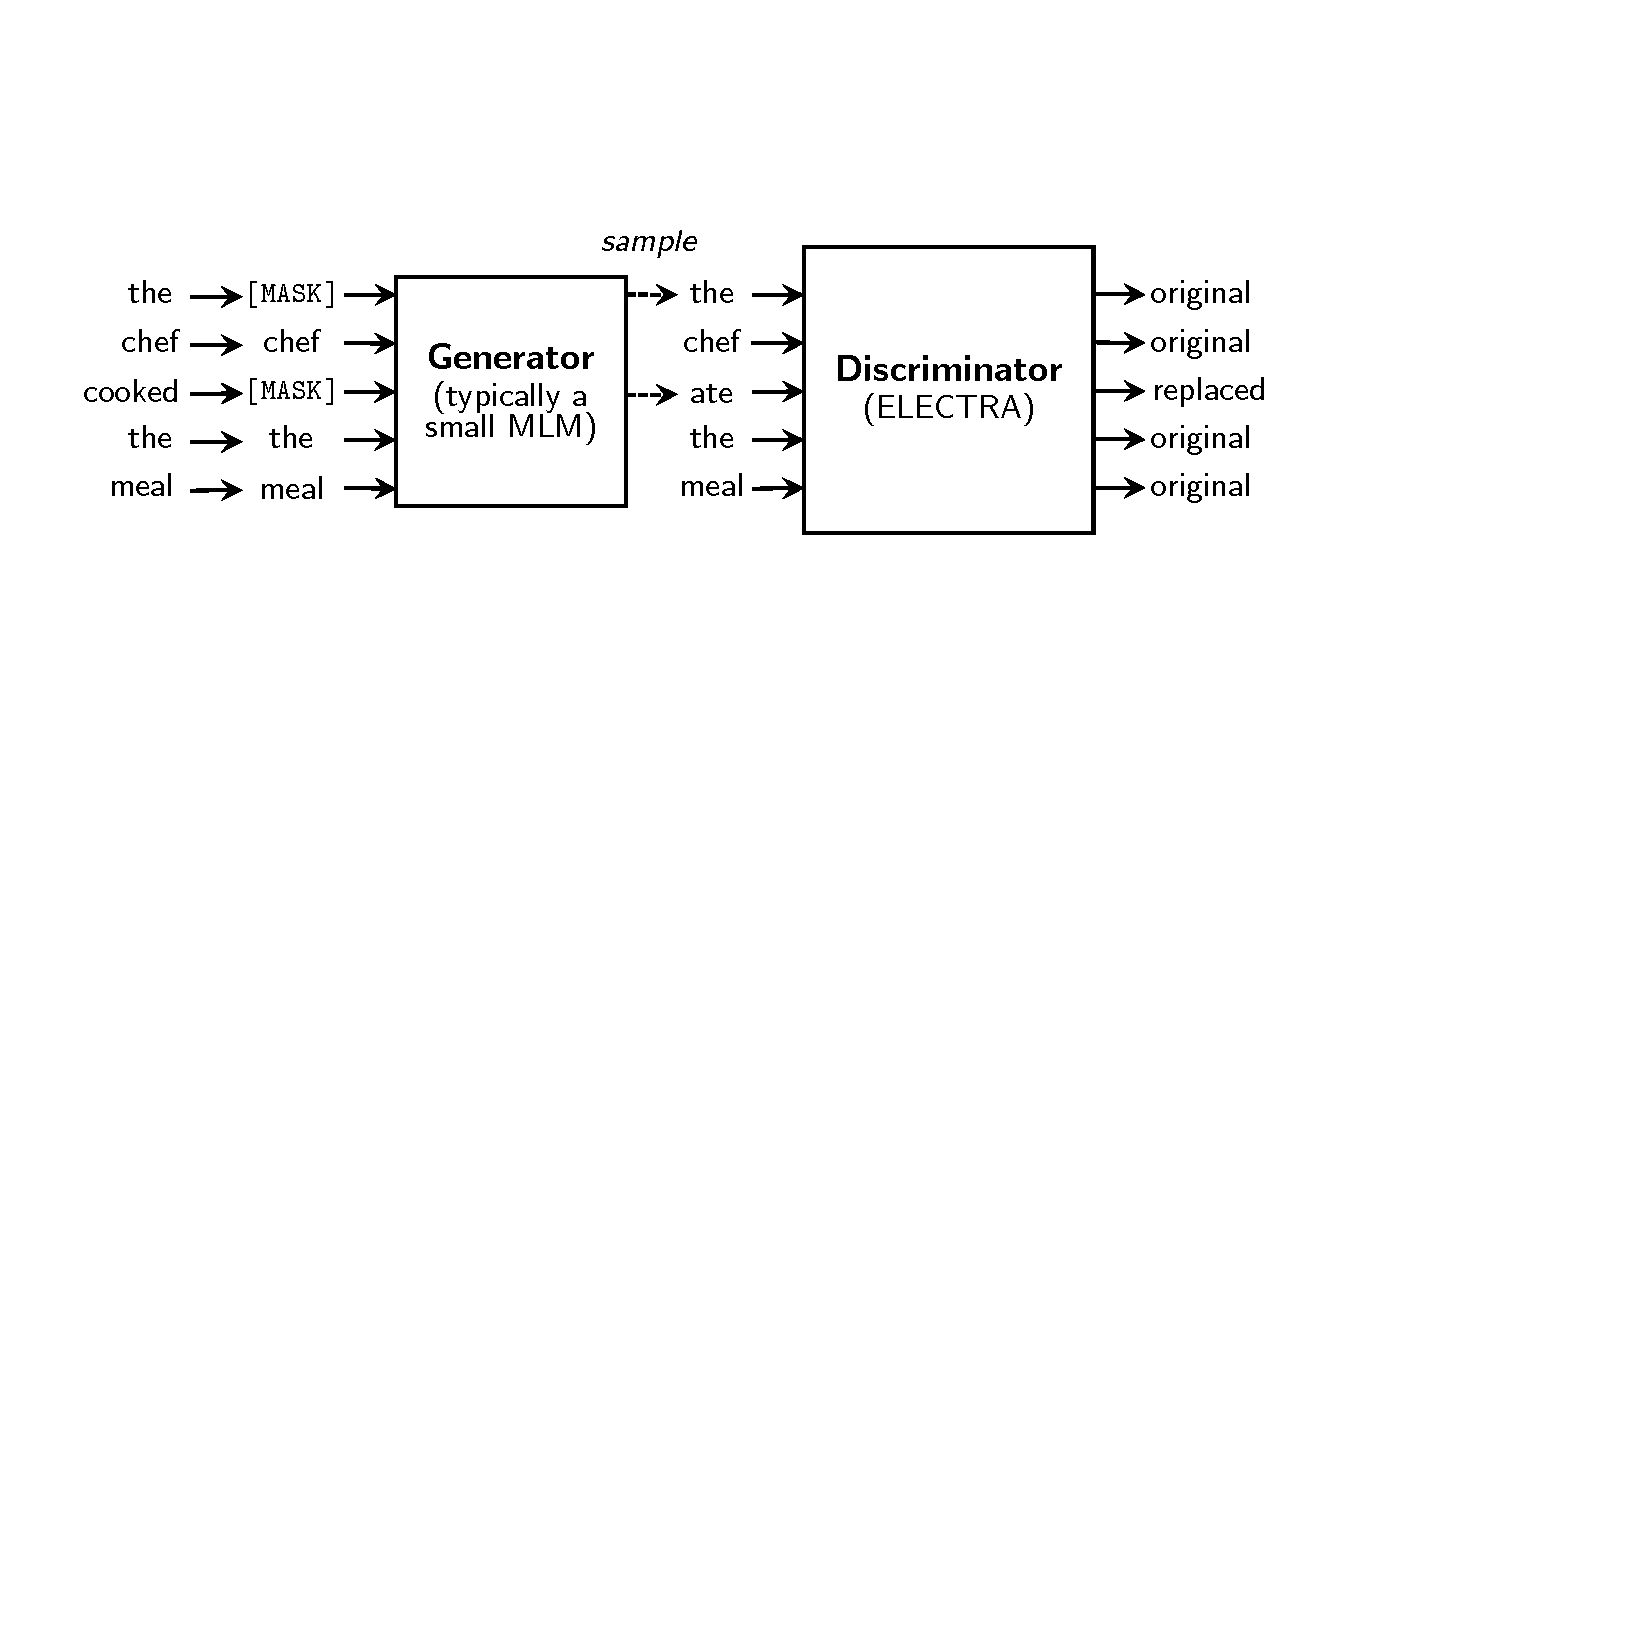
\includegraphics[width=1.0\textwidth]{figures/electra_entr.pdf}
	\end{center}
	\caption{Exemple de la méthode ELECTRA. Figure provenant de \cite{clark2020electrapretrainingtextencoders}.}
	\label{fig:electra}
\end{figure}

Trois éléments rendent l'entraînement du discriminant plus facile.
Premièrement, le générateur dispose de significativement moins de capacité que
le discriminant. En effet, ce dernier contient en général 3 à 4 fois plus de
paramètres (en excluant les couches de projections \textit{embeddings}) que le
générateur. De plus, les entrées du discriminant sont échantillonnées depuis la
distribution engendrée par le générateur, au lieu de sélectionner les entrées
les plus probables selon la distribution du générateur. Finalement, les poids
du générateur sont initialisés aléatoirement et ce dernier est entraîné en même
temps que le discriminant, rendant la tâche de plus en plus difficile au fur et
à mesure que le générateur s'entraîne. Ces trois facteurs rendent la tâche du
discriminant plus facile et permettent de générer des erreurs similaire à ce
que le modèle rencontrera en production.\\

La méthode ELECTRA a été choisie pour deux raisons: c'est une méthode de
préentraînement similaire à la correction d'erreurs dans un texte et la méthode
ELECTRA permet d'augmenter l'efficacité du préentraînement en atteignant des
performances similaires aux performances du MLM en moins d'itérations.


\section{Architecture ELECTRA}
Le modèle ELECTRA utilise une architecture basée sur les modules d'encodeurs
des Transformers \cite{vaswani2023attentionneed}. L'usage d'une architecture
basée sur les transformeur permet d'obtenir une représentation contextuelle
pour tous les jetons d'une séquence. Cette avancée à été marquée par l'arrivée
de \cite{bert},  un modèle Transformers (Bidirectional Encoder Representation
from Transformers). Ce modèle a été développé par Google en 2018 et comprend de
nombreuses versions de différentes tailles et entraînés sur différentes tâches.
Les deux versions canoniques de BERT sont BERT-BASE et BERT-LARGE. Ces deux
versions comprennent respectivement 12 couches et 24 couches, chacune étant
composée de 768 unités de large, divisées en 12 têtes d’attention multiples.
ELECTRA ajoute une nouvelle version plus petite de BERT, dénommée
ELECTRA-small. Celle-ci consiste en 12 couches de 256 unités de large. Ces
modèles à base d'encodeur sont composées de trois parties:
\begin{itemize}
	\item Un \textbf{jetoniseur}, qui s'occupe de traiter le texte entrant et
	      de le convertir un une séquence de d'entiers.
	\item Une \textbf{couche de projection}, qui permet d'associer à chacun des
	      jetons d'entrées une représentation vectorielle qui dépend de la
	      position du jeton dans la séquence ainsi que du jeton lui-même.
	\item Un module d'\textbf{encodeur}, qui permet d'obtenir une
	      représentation contextualisée des entrés. Cette représentation est
	      apprise et varie selon la tâche finale du modèle ainsi que le corpus
	      utiliser pour entraîner le modèle.
\end{itemize}
Notre modèle ELECTRA utilise l'architecture ELECTRA-small.

\section{Affinage pour la détection d'erreurs}
Une fois le modèle ELECTRA préentraîné, il est nécessaire d'adapter le modèle
pour que celui-ci soit en mesure de détecter efficacement les erreurs dans les
textes des utilisateurs. Druide a développé une liste des différents types
d'erreurs, permettant de classifier les différents types d'erreurs en de
grandes catégories, telles que les erreurs de virgules, les erreurs de mots
manquants, les erreurs d'accord du nom, etc. Cette liste contient 750
différents types d'erreurs. Chaque erreur fait partie d'une de ces grandes
catégories, et bon nombre de ces erreurs ont une sous-catégorie, précisant
encore plus le contexte associée à l'erreur. La détection d'erreur est
modélisée comme une tâche de détection d'entité nommée (DEN/NER), dans laquelle
chaque jeton dispose d'un classe. Les classes d'erreurs sont représenté avec un
identifiant, tandis que la classe représentant l'absence d'erreurs est
représenté par l'identifiant $O$. Le modèle à comme objectif de spécifier la
classe de chaque jeton de la séquence. Le schéma $IOB2$ \cite{schemas} est
utilisé pour représenter sans ambiguïté les jetons contigus contenus dans la
même erreur.

\section{Infrastructures en place}
Notre tâche principale consistait à préentraîner un modèle ELECTRA.\@ Or, un
modèle ELECTRA est déjà utilisé pour la tâche de correction en anglais. Ce
dernier n'a pas été préentraîné par Druide. En effet, la librairie
Transformers\cite{wolf-etal-2020-transformers} permet un usage libre de
différents modèles ELECTRA préentraînés. De plus, il existe quelques modèles
ELECTRA préentraînés sur des corpus francophone. Cependant, aucun d'entre eux
ne respectent nos contraintes de tailles et de vitesse. Il est donc nécessaire
d'entraîner un modèle à partir d'un initialisation aléatoire.\\

Nous disposons de deux corpus déjà préparés pour préentraîner et affiner un
modèle Electra. Le corpus de préentraînement est une collection de textes non
structuré provenant de nombreuses sources, notamment des manuels, des articles
de blogues, des livres. Ce corpus de préentraînement est appelé corpus des
Combis et représente 40 gigaoctes (Go) de données et 7 milliard de jetons.
C'est un corpus deux fois plus grand que le corpus de préentraînement utilisé
pour le préentraînement par Google du modèle ELECTRA de même taille. Pour
l'affinage, Druide dispose d'un corpus contenant près de 100000 annotations sur
des textes francophones. Ces annotation sont fournies par Druide et proviennent
d'équipes de linguistes et d'annotateurs corrigeant des textes et classifiant
les erreurs qu'ils y trouvent en fonction des types d'erreurs proposés par
Druide.

\begin{figure}
	\begin{center}
		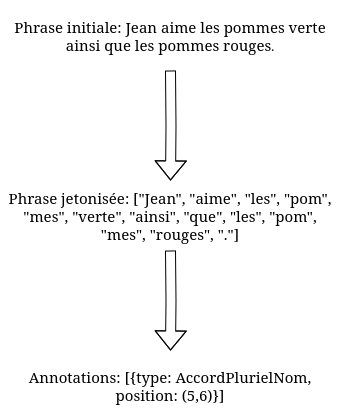
\includegraphics[width=0.4\textwidth]{figures/exemple_annotation.png}
	\end{center}
	\caption{Exemple de texte annoté. Les annotations se font au niveau des jetons et sont donc spécifiques au jetoniseur}
	\label{fig:ex_annotation}
\end{figure}


\chapter{Entraînement de modèles initiaux}
Le préentraînement d'un modèle de langue se fait en trois étapes. Il est
nécessaire de prétraiter les données, de sélectionner un jetonniseur adapté à
la tâche ainsi que d'entraîner le modèle sur la tâche de préentraînement.

\section{Normalisation des données et entraînement d'un jetoniseur}
La normalisation consiste à réduire le nombre de charactèrs différents contenus
dans le corpus. C'est une étape importante puisqu'elle permet de réduire la
taille du vocabulaire du jetoniseur sans pour autant perdre des éléments
syntaxiques. Notre processus de normalisation consistait à tranformer tous les
caractères d'espacement (espaces insécables, tabulations, \textit{U+2002},
etc.) en un même charactère d'espace \textit{U+0020}. La normalisation consiste
aussi en transformer tous les guillements (guillements français, guillemets
informatiques, etc.) en guillemets anglais, de retirer les espaces en trop et
modifier les types d'apostrophes pour que ceux-ci soient uniformes. La
normalisation modifie aussi les espacements entre certains mots. Par exemple,
c'est ainsi que le texte "11 ème étage" devienne "11ème étage".\\

Une fois le texte normalisé, il est possible d'entraîner un jetoniseur adapté à
la tâche. En l'occurence, nous avons initialement sélectionné le jetoniseur
Wordpiece \cite{wu2016googlesneuralmachinetranslation}. C'est le jetoniseur
choisi par les auteurs de l'article de ELECTRA et est actuellement utilisé en
production chez Druide. Il répond donc à nos contraintes. Pour l'entraînement
du jetoniseur, nous utilisons le corpus des combis normalisé, comprenant
environ 40 GO de données. Les hyper-paramètres sélectionnés pour le jetoniseur
wordpiece sont donnés dans le tableau \ref{table:pre-entr-hp}.\\

\section{Préentraînement initial}
Nous préentraînons le modèle à l'aide de l'implémentation originale de ELECTRA.
Celle-ci est disponible au dépôt git suivant:
\url{https://github.com/google-research/electra}. Notre machine dédiée à
l'entraînement dispose de 3 GPUs de 16GB de VRAM chacun. Or, l'implémentation
originale utilise moins de 16GB de VRAM et ne permet pas l'usage de DDP,
limitant la vitesse d'entraînement ainsi que la taille de lot (\textit{batch
	size}). Pour tirer parti au maximum des 3 GPUs disponibles, nous avons
initialisé aléatoirement trois modèle ELECTRA et avons changé l'ordre des
données. En entraînant trois modèles sur le même jeu de données modifié, nous
espérions être en mesure d'appliquer la méthode de la soupe \cite{soup} une
fois les modèles affinés et faire un meilleur usage des ressources
computationnelles à notre disposition. Les hyper-paramètres utilisés durant
l'entraînement des trois modèles sont décrits dans le tableau \ref{table:pre-entr-hp}.
Nous avons divisé par 4 la largeur du générateur, tel que recommandé dans
l'article original de ELECTRA \cite{clark2020electrapretrainingtextencoders}.


\begin{table}[h!]
	\centering
	\begin{tabular}{||c | c c||}
		\hline
		Hyper-paramètres                       & Discriminant & Générateur \\ [0.5ex]
		\hline\hline
		Nombre de couches                      & 12           & 12         \\
		Taille des couches cachées             & 256          & 64         \\
		Taille des couches de projection       & 128          & 128        \\
		Nombre de têtes d'attention            & 4            & 1          \\
		Taille du vocabulaire                  & 30522        & 30522      \\
		Ignore la casse                        & oui          & oui        \\
		\% des jetons masqués                  & -            & 15         \\
		Taux d'apprentissage                   & 5e-4         & 5e-4       \\
		Poids de la perte du générateur        & -            & 1          \\
		Poids de la perte du discriminant      & 50           & -          \\
		Nombre d'itérations de \textit{warmup} & 10000        & 10000      \\
		\hline
	\end{tabular}
	\caption{Hyper-paramètres utilisés pour l'entraînement des modèles}
	\label{table:pre-entr-hp}
\end{table}

Une fois le préentraînement complété, nous avons obtenu les résultats suivants
durant l'évaluation des modèles sur la tâche d'ELECTRA:

\begin{table}[h!]
	\centering
	\begin{tabular}{||c | c c c||}
		\hline
		Métrique                   & Modèle 1 & Modèle 2 & Modèle 3 \\ [0.5ex]
		\hline\hline
		Exactitude du discriminant & 0.952    & 0.949    & 0.950    \\
		AUC du discrimiantn        & 0.934    & 0.929    & 0.934    \\
		Perte du discriminant      & 0.135    & 0.142    & 0.138    \\
		Précision du discriminant  & 0.801    & 0.794    & 0.793    \\
		Rappel du discriminant     & 0.469    & 0.449    & 0.483    \\
		Perte totale               & 8.967    & 9.411    & 9.276    \\
		Exactitude du générateur   & 0.570    & 0.562    & 0.550    \\
		Perte du générateur        & 2.216    & 2.308    & 2.342    \\
		Exactitude du générateur   & 0.469    & 0.458    & 0.448    \\
		\hline
	\end{tabular}
	\caption{Résultats d'évaluation des trois modèles sur la tâche ELECTRA}
	\label{table:respreentrainementsanscasse}
\end{table}
Malgré le changement de l'ordre des données, aucun des trois modèles n'a
performé différemment des autres modèles. Cette remarque nous a poussé à
utiliser la méthode de la soupe \cite{soup} dans le but d'améliorer la
performance du modèle. Cette méthode sera discutée plus en détails dans la
section \ref{chapitre:autretechnique}


\section{Premiers modèles affinés}\label{section:premiersmodelesaffines}
Une fois les trois premiers modèles initaux préentraînés, nous avons entraîné
ces trois modèles sur la tâche de détection des erreurs en français. Les
meilleur métriques enregistrées sont détaillées dans le tableau
\ref{table:premiermodeles} \\

Les mesures F-0.5 obtenues sur l'ensemble de test durant l'affinage sont
contenues dans la figure \ref{fig:3premiermodeles}. Nous utilisons la mesure
F-0.5, dont la formule est données explicitement dans l'équation \ref{eq:f05},
comme principale métrique pour guider nos décisions. Un poids de 0.5 donne deux
fois plus d'importance à la précision par rapport au rappel. Ce choix de
métrique permet de prioriser les modèles qui minimisent les faux positifs et
qui sont donc plus prudents dans leur détection des erreurs.

\begin{equation*} \label{eq:f05}
	F_{0.5}=(1+0.5^2)\frac{\text{précision}\cdot\text{rappel}}{(0.5^2 \cdot \text{précision}) + \text{rappel}}
\end{equation*}


\begin{figure}
	\begin{center}
		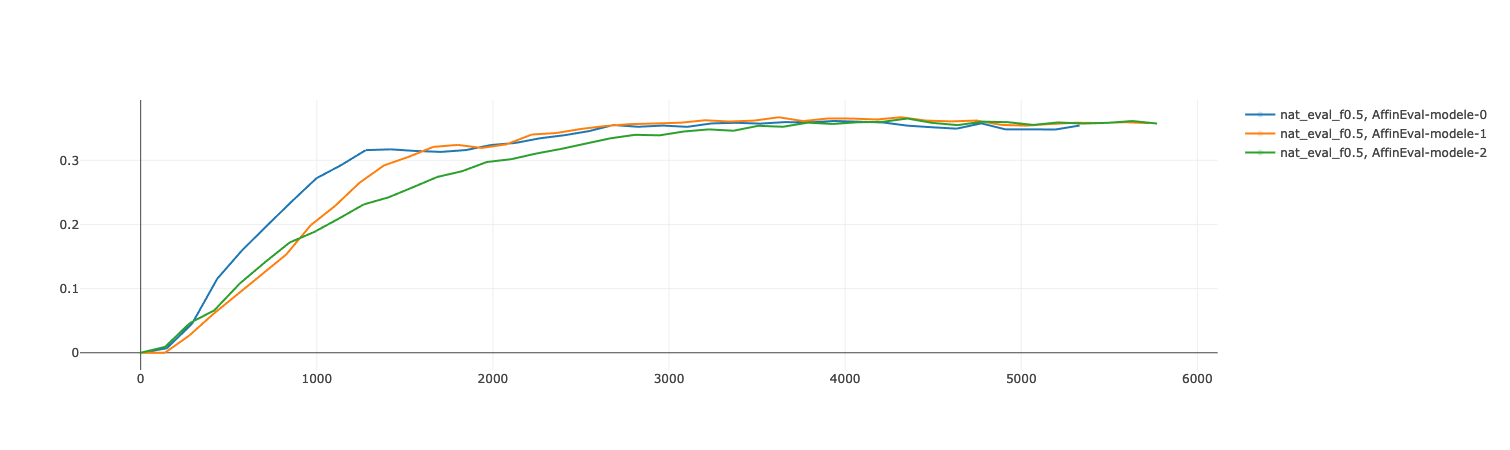
\includegraphics[width=1.40\textwidth]{figures/3premiersmodelesf05.png}
	\end{center}
	\caption{Mesure F-0.5 des trois premiers modèles selon le nombre d'itérations sur données d'évaluation pour la détection d'erreurs en français.}
	\label{fig:3premiermodeles}
\end{figure}

\begin{table}
	\centering
	\begin{tabular}{||c | c | c | c||}
		\hline
		Modèle           & Précision & Rappel & F0.5  \\ [0.5ex]
		\hline\hline
		Modèle initial 1 & 39.59     & 23.84  & 34.97 \\
		Modèle initial 2 & 40.22     & 24.36  & 35.63 \\
		Modèle initial 3 & 39.85     & 24.88  & 35.57 \\
		\hline
	\end{tabular}
	\caption{Résultats des modèles préliminaires sur corpus d'évaluation de la tâche de correction}
	\label{table:premiermodeles}
\end{table}
Tous les modèles ont été entraînés pour avec les hyper-paramètres décrits dans
le tableau \ref{table:affinage-hp}.


\begin{table}
	%% TODO: Mettre à jour les hyper-paramètres d'affinage avec les vraies valeurs
	\centering
	\begin{tabular}{||c | c ||}
		\hline
		Hyper-paramètres                       & Discriminant \\ [0.5ex]
		\hline\hline
		Taux d'apprentissage                   & 12           \\
		Optimisateur                           & 256          \\
		Nombre d'époques                       & 128          \\
		\textit{Weight decay}                  & 4            \\
		Betas de l'optimisateur                & 30522        \\
		Taille de lots                         & 30522        \\
		Nombre d'itérations de \textit{warmup} & 10000        \\
		\hline
	\end{tabular}
	\caption{Hyper-paramètres utilisés pour l'affinage des modèles initiaux}
	\label{table:affinage-hp}
\end{table}

\section{Entraînement d'un modèle avec casse}

Nos premiers modèles prentraînés sont limités en terme de performance par leur
jetoniseur. En effet, le jetoniseur WordPiece entraîné sur les données ignore
la case, et certains types d'erreurs, tel que les majuscules pour les noms
propres, nécessite de connaître la casse des mots. Ce choix n'affecte que peu
la performance du modèle durant le préentraînement, mais pose problème durant
l'affinage sur la tâche de détection des erreurs. Nous avons donc entraîné un
second jetoniseur WordPiece, cette fois-ci sensible à la casse et avec tous les
autres hyper-paramètres identiques. Nous avons par la suite entraîné le modèle
sur l'ensemble des données, encore une fois avec l'ordre des données mélangée
et avec les hyper-paramètres du tableau \ref{table:pre-entr-hp}. Les résultats
du modèle avec casse ainsi que les modèles préliminaires sont contenus dans le
tableau \ref{table:respreentrainementaveccasse}.

\begin{table}[h!]
	\centering
	\begin{tabular}{||c | c c c c||}
		\hline
		Métrique                   & Modèle 1 & Modèle 2 & Modèle 3 & Modèle avec casse \\ [0.5ex]
		\hline\hline
		Exactitude du discriminant & 0.952    & 0.949    & 0.950    & 0.946             \\
		AUC du discrimiantn        & 0.934    & 0.929    & 0.934    & 0.931             \\
		Perte du discriminant      & 0.135    & 0.142    & 0.138    & 0.149             \\
		Précision du discriminant  & 0.801    & 0.794    & 0.793    & 0.795             \\
		Rappel du discriminant     & 0.469    & 0.449    & 0.483    & 0.471             \\
		Perte totale               & 8.967    & 9.411    & 9.276    & 10.31             \\
		Exactitude du générateur   & 0.570    & 0.562    & 0.550    & 0.499             \\
		Perte du générateur        & 2.216    & 2.308    & 2.342    & 2.848             \\
		Exactitude du générateur   & 0.469    & 0.458    & 0.448    & 0.403             \\
		\hline
	\end{tabular}
	\caption{Résultats d'évaluation des trois modèles et du modèle avec casse sur la tâche ELECTRA}
	\label{table:respreentrainementaveccasse}
\end{table}

La performance du discriminant sensible à la cassse est similaire à celles des
autres discriminant. Cependant, le générateur sensible à la casse performe
moins biens que les autres. Une explications possible est que la tâche de
prédire le bon jeton en place en plus difficile avec la casse, puisque les
jetons contenant la casse sont sont souvent syntaxiquement identiques, mais
sont traités comme étant différents durant l'évaluation.\\

Nous avons complété l'affinage du modèle en l'entraînant sur la tâche de
détection des erreurs en français. Nous avons réutilisé les hyper-paramètres
des trois modèles précédents, contenus dans le tableau \ref{table:pre-entr-hp}.
Les résultats du modèle affiné et prenant en compte la casse sont contenus dans
le tableau \ref{table:resaffinagecasse}. Le modèle sensible à la casse performe
mieux que les trois modèle initaux. Cette différence de performance s'explique
par la présence d'erreurs basée sur la casse des mots ainsi qu'un
pré-entraînement plus efficace.

\begin{table}
	\centering
	\begin{tabular}{||c | c | c | c||}
		\hline
		Modèle            & Précision & Rappel & F0.5  \\ [0.5ex]
		\hline\hline
		Modèle initial 1  & 39.59     & 23.84  & 34.97 \\
		Modèle initial 2  & 40.22     & 24.36  & 35.63 \\
		Modèle initial 3  & 39.85     & 24.88  & 35.57 \\
		Modèle avec casse & 42.59     & 25.81  & 37.69 \\
		\hline
	\end{tabular}
	\caption{Résultats des modèles préliminaires sur corpus d'évaluation de la tâche de correction avec le modèle sensible à la casse}
	\label{table:resaffinagecasse}
\end{table}

Les mesures F-0.5 obtenues sur l'ensemble de test durant
l'affinage pour le modèle avec casse sont contenues dans la figure
\ref{fig:f05electraaveccasse}.
\begin{figure}
	\begin{center}
		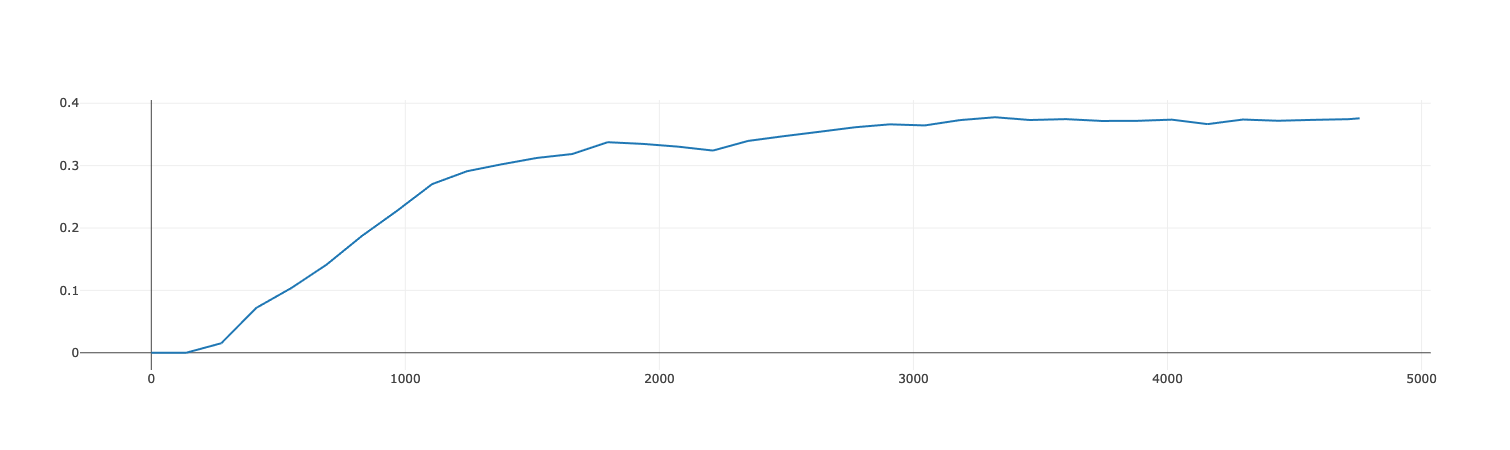
\includegraphics[width=1.0\textwidth]{figures/electraaveccassef05.png}
	\end{center}
	\caption{Mesure F-0.5 du modèle avec casse selon le nombre d'itérations sur
		données d'évaluation pour la détection d'erreurs en
		français.}\label{fig:f05electraaveccasse}
\end{figure}

\section{Comparaison avec CAMEMBERT}
Pour connaître le manque à gagner entre nos petits modèles ELECTRA et des
modèles plus volumineux, nous avons affiné une plus gros modèle et avons
comparé la performances des modèles. Nous avons utilisé CAMEMBERT
\cite{camembert}, un modèle basé sur BERT et préentraîné sur le corpus
francophone OSCAR \cite{oscar} à l'aide de la méthode MLM. CAMEMBERT-base
possède plus de 100 millions de paramètres, le rendant près de 7 fois plus gros
que nos modèle basés sur l'architecture de ELECTRA-small. Ainsi, il est trop
gros pour être déployé dans Antidote. Néanmoins, il offre un possible plafond
quant aux performance que nos modèles peuvent atteindre. \\

Nous avons obtenu la courbe d'entraînement suivante lors de l'affinage de
CAMEMBERT sur la tâche de détection des erreurs en français:

\begin{figure}
	\begin{center}
		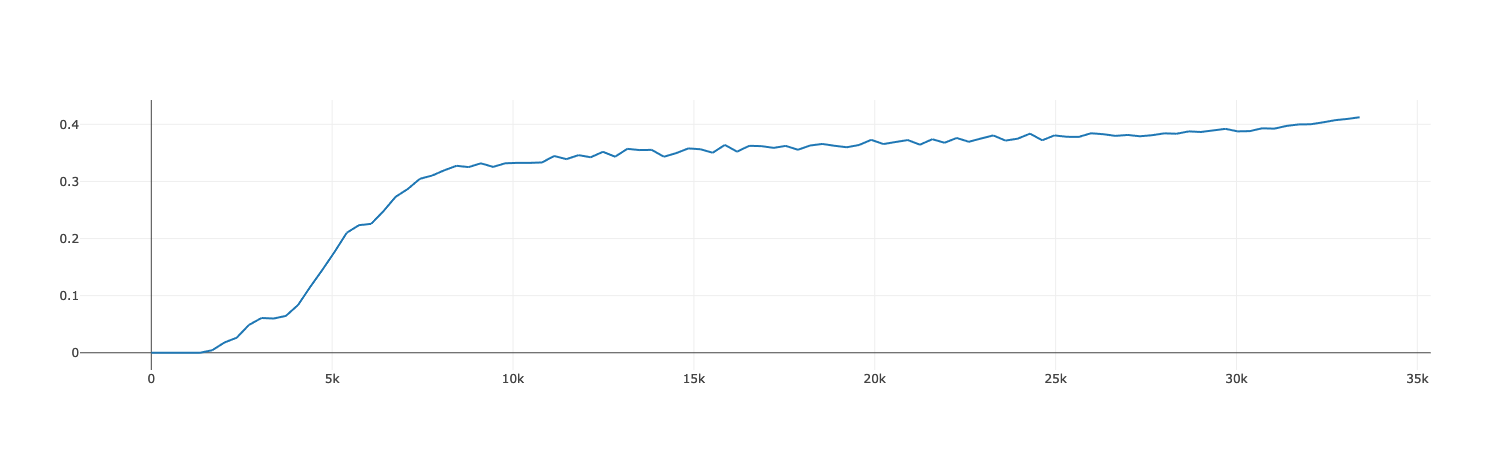
\includegraphics[width=1.0\textwidth]{figures/camembertbasef05100epoquesnat.png}
	\end{center}
	\caption{Mesure F-0.5 de CAMEMBERT selon le nombre d'itérations sur
		données d'évaluation pour la détection d'erreurs en
		français.}\label{fig:f05camembert}
\end{figure}
Le modèle Camembert a atteint une mesure F-0.5 maximale de 40.47, performant
mieux que nos modèles initaux et que le modèle sensible à la casse. La
comparaison complète est disponible dans le tableau
\ref{table:perf_initiaux_camembert}. L'évolution de la performance de Camembert
est disponible dans la figure \ref{fig:f05camembert}. Nous avons limité le
nombre d'époque maximal à 100. Il aurait été intéressant de laisser le modèle
s'entraîner pour plus d'époque et ansi s'assurer que le modèle à atteint sa
performance maximale.

\begin{table}
	\centering
	\begin{tabular}{||c | c | c | c||}
		\hline
		Modèle            & Précision & Rappel & F0.5  \\ [0.5ex]
		\hline\hline
		Modèle initial 1  & 39.59     & 23.84  & 34.97 \\
		Modèle initial 2  & 40.22     & 24.36  & 35.63 \\
		Modèle initial 3  & 39.85     & 24.88  & 35.57 \\
		Modèle avec casse & 42.59     & 25.81  & 37.69 \\
		Camembert-base    & 44.74     & 29.30  & 40.47 \\
		\hline
	\end{tabular}
	\caption{Résultats des modèles préliminaires sur corpus d'évaluation de la tâche de correction avec le modèle sensible à la casse et Camembert}
	\label{table:perf_initiaux_camembert}
\end{table}


%% TODO: insérer citations à camembert et oscar.
%% TODO: Insérer graphique des performances de CAMEMBERT
%% TODO: Mettre à jour tableau des performances de Camembert et les autres modèles



\chapter{Modèle final}\label{chapitre:meilleurmodele}
Notre modèle final consiste en un modèle ELECTRA-small, faisant usage
du jetoniseur de CAMEMBERT. Néanmoins, les augmentations de
performance les plus importants proviennent des deux modifications
suivantes: la recherche d'hyper-paramètres, à l'aide de la librairie
Optuna, et l'ajout d'une phase d'entraînement intermédiaire.
%% TODO: insérer référence à Optuna
\section{Recherche d'hyper-paramètres}
L'un des plus important facteur permettant d'augmenter la performance
de notre modèle final est l'usage de méthode de recherche
d'hyper-paramètres. Nous avons utiliser la librairie Optuna, une
librairie \textit{Python} spécialisée pour la recherche d'hyper-paramètres. En
particulier, nous avons utilisé l'algorithme itératif \textit{TPE}
\cite{watanabe2023treestructuredparzenestimatorunderstanding},
\cite{NIPS2011_86e8f7ab}. Cet algorithme itératif part d'un ensemble
d'hyper-paramèters possibles et tente de trouver la combinaison
maximisant une métrique donnée. Dans notre cas, nous avons utilisé la
mesure f-0.5 comme métrique à maximiser. Nous avons permis à
l'algorithme TPE d'exécuter un maximum de 8 expériences, chacune
faisant usage d'un différent ensemble d'hyper-paramètres. Pour toutes
ces expériences, nous avons permis à l'algorithme \textit{TPE} de
sélectionner la valeur des hyper-paramètres suivants:
\begin{itemize}
	\item Taille des lots durant la phase d'entraînement
	\item \textit{Weight decay} de l'optimisateur
	\item Taux d'apprentissage
\end{itemize}
Cette recherche d'hyper-paramètres requiert un affinage complet du
modèle pour chaque expérience et est donc trop dispendieux pour être
utilisé à grande échelle. Néanmoins, la recherche d'hyper-paramètres à
permis d'établir un nouveau record sur la tâche de correction en
français, augmentant la F-mesure à 41,23.

% TODO: Ajouter cette section les hyper-paramèters sont disponibles
% \subsection{Remarques sur les hyper-paramètres}
% Durant les affinages sur la tâche de correction neuronale, nous avons
% noté la tendance du modèle à sélectionner les hyper-paramètres

\subsection{Note sur la qualité des données d'affinage}
La recherche d'hyper-paramètres a révélé une tendance intéressante:
les modèles gagnent à avoir une très petite taille de lot
(\textit{batch size}) lors de leur entraînement. En effet, les modèles
performant le mieux ont obtenus leur meilleure performance en
utilisant une taille de lot de 8. Cette observation offre un contraste
drastique entre les méthodes d'entraînement contemporaines pour les
modèles de langue, qui font souvent usage d'une très grande taille de
lot. Une raison souvent données pour expliquer les meilleures
performances des modèles entraînés avec une grande taille de lot est
qu'une taille de lot plus grande offre une plus grande résistance
quant aux exemples bruités, contenant des erreurs ou plus généralement
de mauvaise qualité. Or, la meilleure performance des modèles
utilisant une petite taille de lot s'explique par la qualité des
données annotés. En effet, les exemples contenus dans le corpus de
test sont annotés par des humains formés pour une telle tâche, et les
textes sont basés sur des corpus filtrés des humains, bien souvent des
linguistes.

\section{Phase d'entraînement intermédiaire}
Le plus gros gain de performance enregistré durant l'entraînement, en
terme de mesure f-0.5 est l'ajout d'une phase d'entraînement
intermédiaire. Cette phase additionnelle a rendu l'entraînement plus
stable ainsi qu'augmenté la performance du modèle final.

\subsection{Collecte et extraction des données}
Nous avons été en mesure d'augmenter les données annotés à l'aide des
corrections des utilisateurs. L'application Antidote dispose d'une version
Web. Celle-ci est établie depuis de nombreuses années et collecte les données
anonymisées des utilisateurs. Cette base de données comporte notamment les
phrases anonymisée entrée par les utilisateurs de Antidote Web, ainsi que les
phrases corrigées correspondantes et les correctins proposées par Antidote
qui ont été acceptées par les utilisateurs. Ainsi, les faux positifs proposés
par antidote sont potentiellement ignorés par utilisateurs et ne font donc pas
partie du nouveau corpus.
%% TODO: Refaire la formulation de cette phrase:
Après l'extraction des données, nous avons traiter ces nouvelles données pour
que ces derniers soit compatibles avec notre méthodologie d'entraînement. Nous
avons nettoyer le corpus en retirant les corrections ne faisant par partie de
la liste de corrections utilisées dans l'affinage. Ce nouveau corpus contient un
total de 3.5 millions de phrases annotés provenant des utilisateurs et corrigés
par Antidote. Ce nouveau corpus est ainsi 35 fois plus grand que le corpus
d'affinage initial, qui contient 100000 corrections faites par des linguistes.
\subsection{Résultat de la phase intermédiaire}
Nous avons utilisé ce nouveau corpus comme un tâche intermédiaire. Celle-ci est exécutée après le pré-entraînement et après l'affinage du modèle. Cette nouvelle phase intermédiaire s'est avérée être très importante pour la performance du modèle sur la correction des erreurs en français. Nous avons observé une augmentation de près de 5 points de mesure F-0.5 ainsi qu'une hausse importante dans la vitesse à laquelle les modèles convergent:

\begin{figure}
	\begin{center}
		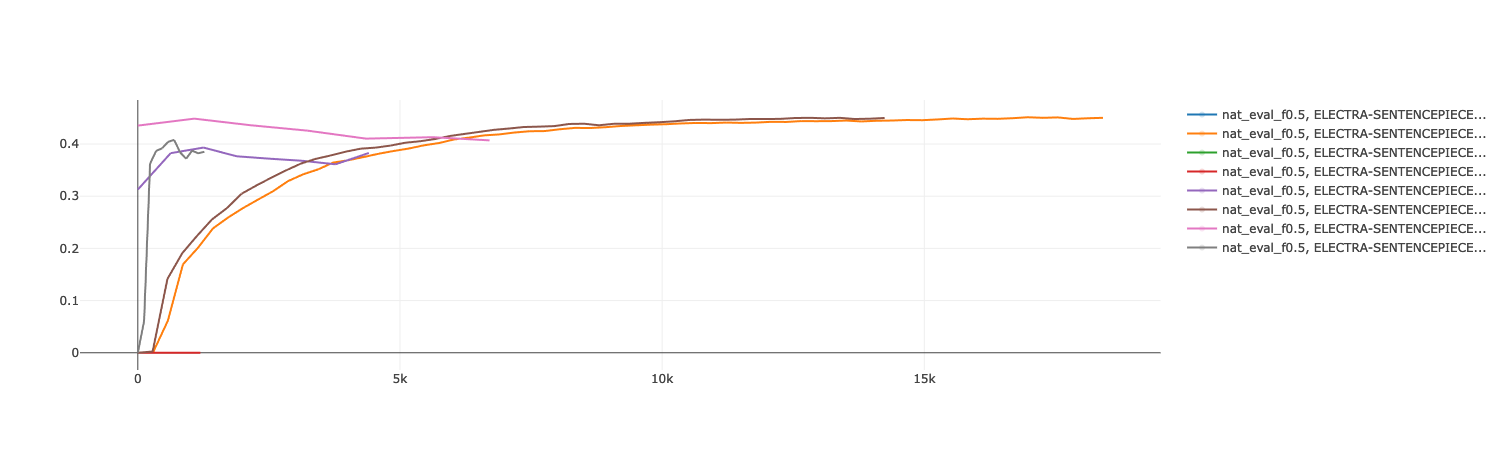
\includegraphics[width=1.0\textwidth]{figures/electrasentencepieceawebf05optuna.png}
	\end{center}
	\caption{Mesures F-0.5 des modèles ELECTRA avec SentencePiece sur la détections des erreurs en français, avec l'ajout de la tâche intermédiaire. Les différentes courbes correspondent à différentes expériences faites à l'aide d'Optuna. L'axe des 5 représente le nombre d'itérations et l'axe horizontal représente la mesure F-0.5.}\label{fig:electraaweb}
\end{figure}


\begin{figure}
	\begin{center}
		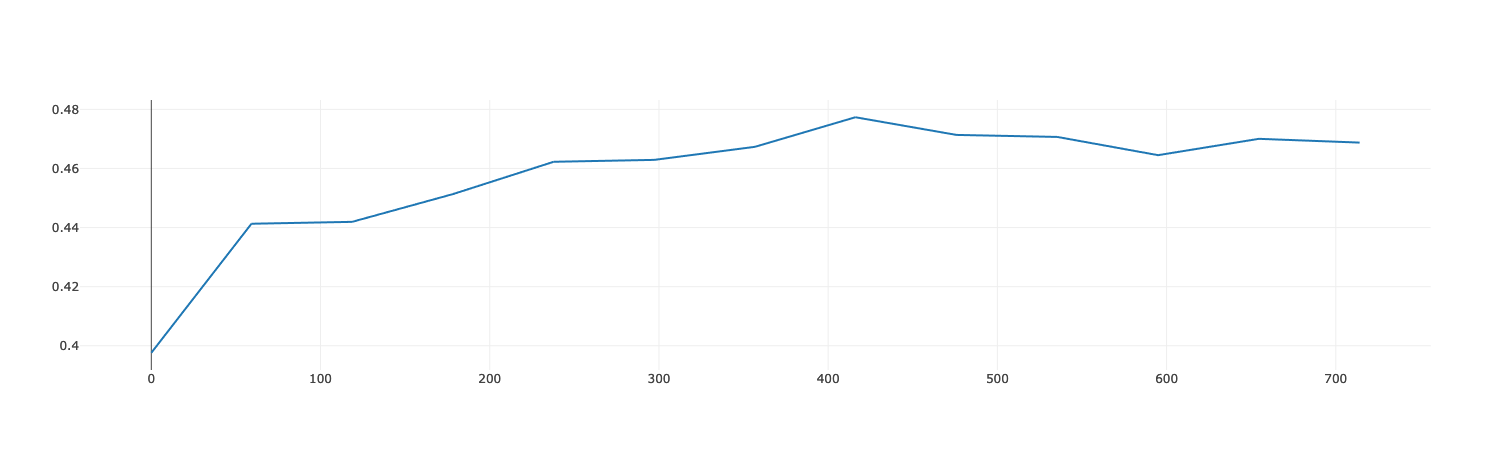
\includegraphics[width=1.0\textwidth]{figures/meilleurmodelenatf05.png}
	\end{center}
	\caption{Courbe de la mesure F-0.5 durant l'affinage du modèle final. Ce dernier correspond au meilleur modèle et utilise l'architecture ELECTRA. De plus, ce modèle a été entraîné avec la phase intermédiaire et utilise le jetoniseur SentencePiece.}\label{fig:meilleurmodeleaweb}
\end{figure}
Il est intéressant de noter la diminution du temps avant d'atteindre la
convergence. En effet, les modèles initaux (figure \ref{fig:3premiermodeles})
débutent leur affinage avec une mesure F-0.5 de 0, tandis que le modèle final
débute son affinage avec une mesure F-0.5 de près de 0.4. De plus, le nouveau
modèle obtient une meilleure performance finale, telle qu'indiqué dans le tableau des
résultats \ref{table:resultatfinaux}.
%%TODO: Mettre à jour le tableau des résultats finaux
\begin{table}
	\centering
	\begin{tabular}{||c | c||}
		\hline
		Modèle           & F0.5  \\ [0.5ex]
		\hline\hline
		Modèle initial 1 & 34.97 \\
		Modèle initial 2 & 35.63 \\
		Modèle initial 3 & 35.57 \\
		\hline
	\end{tabular}
	\caption{Résultats finaux des modèles sur corpus d'évaluation de la tâche de correction}
	\label{table:resultatfinaux}
\end{table}

\chapter{Autres techniques} \label{chapitre:autretechnique}
La plupart des techniques mise en oeuvre durant ma recherche n'ont pas eu
données les résultast escomptés. Cette section contient les résultats de ces
différentes techniques qui n'ont pas améliorée la performance des modèles. Ces
techniques y seront brièvement abordées.
\section{Soupe}
Nous avons appliqué la méthode Soupe (de l'anglais \textit{Soup}) \cite{soup},
qui consiste en une somme pondérée des poids des paramètres des différents
modèles. Cette méthode permet simple permet d'augmenter la performance de
modèles affinés sans pour autant faire usage de beaucoup de ressources et sans
augmenter le temps d'inférence. L'intuition derrière cette technique est qu'un
meilleur modèle se trouve souvent entre plusieurs modèles affinés. Donc, si nos
modèles utilisés pour faire la soupe sont à proximité d'un minimum local pour
une fonction de perte donnée, alors la moyenne arithmétique des poids des
modèles pourrait résuler en un modèle dont la perte est plus proche de l'optimum
local.\\
\\
Nous avons fait une soupe à partir de nos 3 premiers modèles affinés, décris dans
la section \ref{section:premiersmodelesaffines}. Nous avons par la suite affiné
notre soupe sur la tâche de détection des erreurs. Malheureusement, notre modèle
n'a jamais été en mesure de converger durant l'affinage. Une explication
possible est qu'au moins une de nos trois modèles affinés convergeait vers un
optimum local différent. Ainsi, l'initialisation du modèle soupe était éloignée
des optimums locaux des modèles.
\section{Nettoyage des données}
Une part éssentielle de l'entraînement est de fournir des données de qualité
à notre modèle. Or, une partie importante du corpus de pré-entraînement est
de piètre qualité. En effet, les données proviennent de plusieurs types de
sources différentes: livres, revues, article de blogue et site internet. Toutes
ces sources ne sont pas sans erreurs ou ne contiennent pas nécessairement des
textes avec un niveau de langue suffisant. C'est pourquoi retirer les exemples
de piètre qualité est importants. Or, le nettoyage d'un corpus de grande
taille nécessite l'usage d'heuristiques de sélection. Pour la création du
pipeline de nettoyage, nous avons utiliser la librarie \textit{Datatrove} de
\textit{HuggingFace} \cite{penedo2024datatrove} et l'avons modifié pour qu'elle
convienne à notre usage.\\
\\
Nous avons appliqués principalement 4 filtres, dont l'ordre d'apparition est le suivant:
\begin{itemize}
	\item Filtre de longueur
	\item Filtre de langue
	\item Filtre de Gopher
	\item Filtre de C4
\end{itemize}
Le filtre de longueur retire les exemples qui contiennent moins de 6 mots
et Le filtre de langue retire les exemples qui ne sont pas en français. Ce
dernier fait usage d'un modèle FastText \cite{joulin2016fasttext} pour détecter
la langue du texte. Le filtre Gopher est plus complexe et utilises plusieurs
heuristiques pour filtrer le contenu du corpus:
\begin{itemize}
	\item La longueur de l'exemple est supérieure à 100000 mots et inférieure à 5 mots
	\item La proportion de lettres parmi l'exemple est inférieure à 70\%
	\item La proportion de symboles parmi les mots est supérieure à 10\%
	\item Le nombre de \textit{stop words} est inférieur à 2
\end{itemize}
Finalement, le filtre C4 retire les exemples contenant du JavaScript, le terme
\textit{Lorem Ipsum}, le symbole $\{$  ou encore les exemples contenant des
conditions d'utilisations.\\
Les filtres ont retiré près de 23\% du contenu total initial du corpus: des  314
907 209 exemples initiaux, il en reste 242 710 245 dans le corpus nettoyé. Les
différents filtres ont eu un impact variable sur le résultat final:
\begin{itemize}
	\item filtre de longueur: retiré 38 585 180 exemples
	\item filtre de langue: retiré 8 283 109 exemples
	\item Gopher: retiré 25 228 530 exemples
	\item C4: retiré 14 741 exemples
\end{itemize}
Après le nettoyage du corpus, nous avons entraîné une nouvelle fois un modèle,
mais cette fois-ci sur le corpus restreint. Nous avons utilisé les mêmes
hyper-paramètres que le meilleur modèle décrit au chapitre
\ref{chapitre:meilleurmodele} durant le pré-entraînement et la phase
intermédiaire, puis avons effectué une recherche d'hyper-paramètres à l'aide
d'Optuna. La figure \ref{fig:electrapropre} montre les courbe de mesure F-0.5
durant la recherche d'hyper-paramètre sur la tâche de détection des erreurs
en français.
% TODO: Ajouter une explication quant à la différence de performance. Données
% court sont pertinents, permettent de réguler le modèle?

\begin{figure}
	\begin{center}
		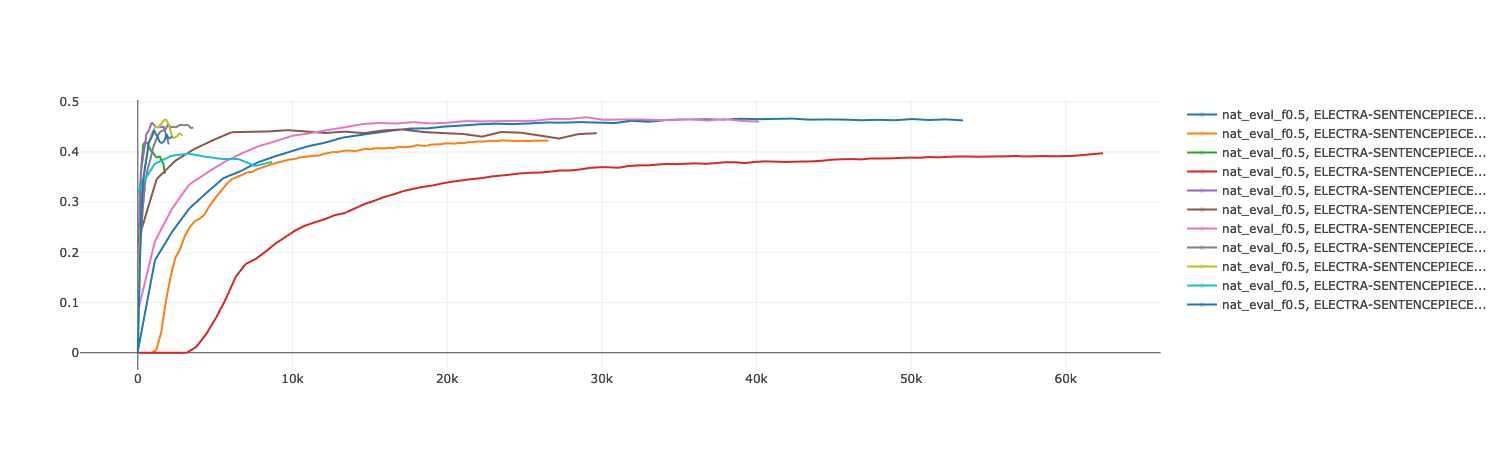
\includegraphics[width=1.0\textwidth]{figures/electrasentenecepicepropreoptunaf05.png}
	\end{center}
	\caption{Mesure F-0.5 durant la recherche d'hyper-paramètres après avoir pré-entraîné sur le corpus nettoyé. Aucun des modèle n'atteint la performance du modèle final (\ref{fig:meilleurmodeleaweb})}
	\label{fig:electrapropre}
\end{figure}

%% TODO: Discuter de Fast-Electra si suffisament de place
% \section{Fast-ELECTRA}
%% TODO: Discuter de MOE si suffisament de place
% \section{Architecture hybrides à base de MOE}
\chapter{Conclusions}
Durant ce stage, je me suis familiarisé avec les principales étapes du
développement d'un système en traitement automatique de la langue. J'ai
travaillé sur le nettoyage et traitement des données, le prototypage de
différents modèles ainsi que l'évaluation des modèles d'aprentissage
automatique. De plus, nous avons appris à connaître l'écosystème
d'apprentissage automatique en \textit{Python} ainsi que les modèles considérés
comme l'état de l'art en traitement automatique des langues.

Nous avons obtenu de bons résultats préliminaires, notamment en ajoutant une
phase intermédiaire durant l'entraînement et en effectuant une recherche
d'hyper-paramètre. Nous pensons qu'une avenue d'amélioration du modèle
consisterait à faire usage de grands modèles de langues dans le but de générer
des données artificielles de bonnes qualité. En particulier, une stratégie qui
pourrait être intéressante pour augmenter la performance du modèle serait
d'utiliser un grand modèle de langue pour générer des phrases comportant des
erreurs dans le but d'augmenter la taille du corpus d'entraînement. Il serait
particulièrement intéressant de générer des données artificielles pour les
types d'erreurs avec lesquels notre modèle à encore de la difficulté. Cela
permettrait de réduire le coût et le temps de génération des phrases
artificielles et permettrait d'avoir un modèle plus performant sur tous les
types d'erreurs présent dans la liste des erreurs corrigés par Antidote.

%% TODO: Discuter des directions futures: Génération de données artificielles
%%--------------%
%%     index    %
%%--------------%

%% S'il y a lieu, décommenter la ligne pour mettre votre index

%%\printindex

%%------------------------------------------------- %
%%         références --- bibliographie             %
%%------------------------------------------------- %
% Enlever les commentaires de la prochaine commande si vous préférez que le
% chapitre s'appelle « Références » plutôt que « Bibliographie » (au choix selon le contexte).
%%\let\bibname=\refname

%% Lorsque vous serez prêt à faire afficher votre bibliographie
%% et vos références, enlevez les commandaires des commandes suivantes
%% et donnez le nom de votre fichier .bib à la commande \bibliography{..}
%% (consultez l'exemple au besoin).  Vous pouvez utiliser le style de votre
%% choix.
\bibliographystyle{amsplain-french}     % Le style de la bibliographie. Notons que
% les extensions ne sont pas données pour ces deux fichiers.
\def\bibname{R\'ef\'erences} % Nom obligatoire de la section des références.
% On utilise \'e car le é cause des problèmes
% dans la table des matière
%% ENGLISH
%\def\bibname{References}
\bibliography{ref}     % La base de données contenant des entrées bibliographiques.
% Seules celles référencées dans le texte seront ajoutées
% \`a la bibliographie.

%%------------------------------------------------- %
%%                  Annexe A                        %
%%------------------------------------------------- %

\end{document}



\endinput
%%
%% End of file `gabaritmem.tex'.
